\documentclass[12pt,letterpaper]{hmcpset}
\usepackage[margin=1in]{geometry}
\usepackage{graphicx}
\usepackage{amsmath}
\usepackage{multirow}

% info for header block in upper right hand corner
\name{}
\class{Math 35 - Section }
\assignment{Homework 2}
\duedate{Tuesday, November 3, 2015}

\newcommand{\pn}[1]{\left( #1 \right)}
\newcommand{\abs}[1]{\left| #1 \right|}
\newcommand{\bk}[1]{\left[ #1 \right]}
\newcommand{\vc}[1]{\left\langle #1 \right\rangle}

\renewcommand{\P}[1]{P \left( #1 \right)}

\begin{document}

\problemlist{2.1.\{ 3, 5 \}, 2.2.\{19, 21, 28 \}, 2.3.\{ 35, 40 \}, 2.4.\{45, 52, 67 \}, 2.5.\{74, 80\}}

% 2.1.3 %
\begin{problem}[2.1.3]
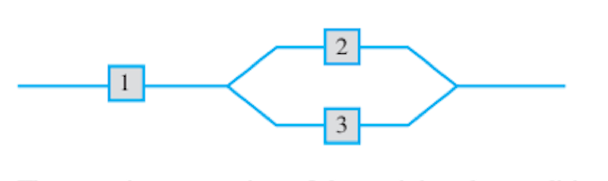
\includegraphics[scale=1]{Nov_3_1.png}\\
    Three components are connected to form a system as shown in the diagram. Because the components in the 2-3 subsystem are connected in parallel, that subsystem will function if at least one of the two individual components functions. For the entire system to function, component 1 must function and so must the 2-3 subsystem.\\ \\
    The experiment consists of determining the condition of each component [S (success) if functional and F (failure) if not].
\\ \\
(a) Which outcomes are contained in the event A that exactly two out of the three components function?
\\
(b) Which outcomes are contained in the event B that at least two of the components function?
\\
(c) Which outcomes are contained in the event C that the system functions?
\\
(d) List outcomes in $C^\prime$, and A $\cup$ C, A $\cap$ C, B $\cup$ C, and B $\cap$ C.

\end{problem}

\begin{solution}

\end{solution}
\newpage

% 2.1.5 %
\begin{problem}[2.1.5]

A family consisting of three persons, – A, B, and C – goes to a medical clinic that always has a doctor at each of the stations 1, 2, and 3. During a certain week, each member of the family visits the clinic once and is assigned at random to a station. The experiment consists of recording the state number for each member. One outcome is (1, 2, 1) for A to station 1, B to station 2, and C to station 1. 
\\ \\
(a) List the 27 outcomes in the sample space.
\\
(b) List all outcomes in the event that all three members go to the same station.
\\
(c) List all outcomes in the event that all members go to different stations:
\\
(d) List all outcomes in the event that no one goes to station 2:



\end{problem}

\begin{solution}
(a) Let sample space be represented as $S$.

\end{solution}
\newpage

% 2.2.19 %
\begin{problem}[2.2.19]
Human visual inspection of solder joints on printed circuit boards can be very subjective. In one batch of 10,000 joints, inspector A found 724 that were judged defective, inspector B found 751 such joints, and 1159 of the joints were judged defective by at least one of the inspectors. Suppose that one of the 10,000 joints is randomly selected.
\\ \\
(a) What is the probability that the selected joint was judged to be defective by neither of the two inspectors?
\\
(b) What is the probability that the selected joint was judged to be defective by inspector B but not by inspector A?


\end{problem}

\begin{solution}

\end{solution}
\newpage
% 2.2.21 %
\begin{problem}[2.2.21]
An insurance company offers four different deductible levels -- none, low, medium, and high -- for its homeowner’s policyholders. The accompanying table gives proportions for the various categories of policyholders who have both types of insurance. For example, the proportion of individuals with both low homeowner’s deductible and low auto deductible is 0.06 (6$\%$ of all such individuals).\\
\begin{center}
	\begin{tabular}{|c||c|c|c|c|}
		\hline
		  & \multicolumn{4}{c|}{Homeowner}\\
 		\hline
 		\hline
 		Auto & N & L & M & H \\
 		\hline
 		L & 0.04 & 0.06 & 0.05 & 0.03 \\
 		M & 0.07 & 0.10 & 0.20 & 0.10\\
 		H & 0.02 & 0.03 & 0.15 & 0.15\\
 		 \hline
	 \end{tabular}

\end{center}
Suppose an individual having both types of policies is randomly selected.
\\ \\
(a) What is the probability that the individual has a medium auto deductible and a high homeowner’s deductible?
\\
(b) What is the probability that the individual has a low auto deductible? A low homeowner’s deductible?
\\
(c) What is the probability that the individual is in the same category for both auto and homeowner’s deductibles?
\\
(d) Based on your answer in part (c), what is the probability that the two categories are different?
\\
(e) What is the probability that the individual has at least one low deductible level?
\\
(f) Using the answer in part (e), what is the probability that neither deductible level is low?



\end{problem}

\begin{solution}

\end{solution}
\newpage

% 2.2.28 %
\begin{problem}[2.2.28]
In Exercise 5 (see above), suppose that any incoming individual is equally likely to be assigned to any of the three stations irrespective of where other individuals have been assigned. What is the probability that:
\\ \\
(a) All three family members are assigned to the same station?
\\
(b) At most two family members are assigned to the same station?
\\
(c) Every family member is assigned to a different station?

\end{problem}

\begin{solution}

\end{solution}
\newpage
% 2.3.35 %
\begin{problem}[2.3.35]
(35) A production facility employs 10 workers on the day shift, 8 workers on the swing shift, and 6 workers on the graveyard shift. A quality control consultant is to select 5 of theses workers for in-depth interviews. Suppose the selection is made in such a way that any particular group of 5 workers has the same chance of being selected as does any other group.
\\ \\
(a) How many selections result in all 5 workers coming from the day shift? What is the probability that all 5 selected workers will be from the day shift?
\\
(b) What is the probability that all 5 selected workers will be from the same shift?
\\
(c) What is the probability that at least two different shifts will be represented among the selected workers?
\\
(d) What is the probability that at least one of the shifts will be unrepresented in the sample of workers?

\end{problem}

\begin{solution}

\end{solution}
\newpage
% 2.3.40 %
\begin{problem}[2.3.40]
Three molecules o type A, three of type B, three of type C, and three of type D are to be linked together to form a chain molecule. One such chain molecule is ABCDABCDABCD, and another is BCDDAAABDBCC.
\\
(a) How many such chain molecules are there? [Hint: If the three A’s were distinguishable from one another – A1, A2, A3 – and the B’s, C’s, and D’s were also, how many molecules would there be? How is this number reduced when the subscripts are removed from the A’s?]
\\
(b) Suppose a chain molecule of the type described is randomly selected. What is the probability that all three molecules of each type end up next to one another (such as in BBBAAADDDCCC)?

\end{problem}

\begin{solution}

\end{solution}
\newpage

% 2.4.45 %
\begin{problem}[2.4.45]
The population of a particular country consists of three ethnic groups. Each individual belongs to one of the four major blood groups. The accompanying $\textit{joint probability table}$ gives the proportions of individuals in the various ethnic group-blood group combinations.\\
\begin{center}
	\begin{tabular}{|c||c|c|c|c|}
		\hline
		  & \multicolumn{4}{c|}{Blood Group}\\
 		\hline
 		\hline
 		Ethnic Group & O & A & B & AB \\
 		\hline
 		1 & 0.082 & 0.106 & 0.008 & 0.004 \\
 		2 & 0.135 & 0.141 & 0.018 & 0.006\\
 		3 & 0.215 & 0.200 & 0.065 & 0.020\\
 		 \hline
	 \end{tabular}

\end{center}
Suppose that an individual is randomly selected from the population, and define events by $A$ = {type A selected}, $B$ = {type B selected}, and $C$ = {ethnic group 3 selected}.
\\ \\
(a) Calculate $P(A)$, $P(C)$, and $P(A\cap C)$.
\\
	(b) Calculate both $P(A|C)$ and $P(C|A)$, and explain in context what each of these probabilities represents.
\\
(c) If the selected individual does not have type B blood, what is the probability that he or she is from ethnic group 1?

\end{problem}

\begin{solution}

\end{solution}
\newpage

% 2.4.52 %
\begin{problem}[2.4.52]
A system consists of two identical pumps, $\#$1 and $\#$2. If one pump fails, the system will still operate. However, because of the added strain, the remaining pump is now more likely to fail than was originally the case. That is, $r = P$($\#$2 fails$|\#1$ fails) $> P$($\#$2 fails) $= q$. If at least one pump fails by the end of the pump design life in 7$\%$ of all systems and both pumps fail during that period in only 1$\%$, what is the probability that pump $\#$1 will fail during the pump design life?
\\ \\
(a) How many such chain molecules are there? [Hint: If the three A’s were distinguishable from one another – A1, A2, A3 – and the B’s, C’s, and D’s were also, how many molecules would there be? How is this number reduced when the subscripts are removed from the A’s?]
\\
(b) Suppose a chain molecule of the type described is randomly selected. What is the probability that all three molecules of each type end up next to one another (such as in BBBAAADDDCCC)?

\end{problem}

\begin{solution}

\end{solution}
\newpage

% 2.4.67 %
\begin{problem}[2.4.67]
Suppose a particular surveillance system has a 99$\%$ chance of correctly identifying a future terrorist and a 99.9$\%$ chance of correctly identifying someone who is not a future terrorist. If there are 1000 future terrorists in a population of 300 million, and 1 of these 300 million is randomly selected, scrutinized by the system, and identified as a future terrorist, what is the probability that he/she is actually a future terrorist? Does the value of this probability make you uneasy about the surveillance system?

\end{problem}

\begin{solution}

\end{solution}
\newpage

% 2.5.74 %
\begin{problem}[2.5.74]
The proportions of blood phenotypes in the U.S. population are as follows.\\
\begin{center}
	\begin{tabular}{c|c|c|c}
 		A & B & AB & O \\
 		\hline
 		0.40 & 0.11 & 0.04 & 0.45
	 \end{tabular}
\end{center}
Assuming that the phenotypes of two randomly selected individuals are independent of one another, what is the probability that both phenotypes are O? What is the probability that the phenotypes of tow randomly selected individuals match?
\end{problem}

\begin{solution}

\end{solution}
\newpage

% 2.5.80 %
\begin{problem}[2.5.80]
Consider the system of components connect as in the accompanying picture.
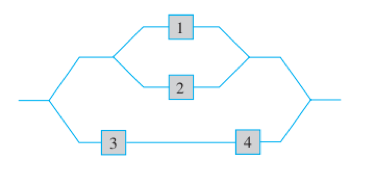
\includegraphics[scale=1]{Nov_3_2.png}\\
    Components 1 and 2 are connected in parallel, so that subsystem works iff either 1 or 2 works; since 3 and 4 are connected in series, that subsystem works iff both 3 and 4 work. If components work independently of one another and P(component $i$ works) = .9 for $i$ = 1, 2 and = .8 for $i$ = 3, 4, calculate P(system works).
\\
\end{problem}

\begin{solution}

\end{solution}

\end{document}
